\documentclass[10pt, a4paper]{beamer}

\usetheme{Berkeley}
\usepackage{subcaption}
\usecolortheme{sidebartab}

\begin{document}
	\setbeamertemplate{sidebar left}{}
	\title{Progress Presentation-I}
	\subtitle{e-Yantra Summer Intership-2016 \\ Object Tracking Camera for Autonomous Drone}
	\author{Abhishek Rathore\\ Gopineedi Harsha Vardhan\\
	\textbf{Mentors:}\\Akshat Jain\\Pushkar raj\\Rama kumar\\Santosh}
	\institute{IIT Bombay}
	\date{\today}
	%\addtobeamertemplate{sidebar left}{}{\includegraphics[scale = 0.3]{logowithtext.png}}
	\frame{\titlepage}

\setbeamertemplate{sidebar left}[sidebar theme]
\section{Overview of Project}
\begin{frame}{Object Tracking Camera for Autonomous Drone}
	\begin{itemize}
		\item Nowadays, we get drones that say they are tracking objects. But what they actually use is the GPS location of your mobile phone. So basically what the drone is tracking is the phone and not the actual object/human. This was the reason we came up with this idea of making an Object Tracking Camera system that can be mounted on an autonomous drone. This system will track an object using Real-Time Image Processing.
		\end{itemize}
\end{frame}
\begin{frame}{Object Tracking Camera for Autonomous Drone}
  \begin{itemize}
		\item \textbf{Objective}
		   \begin{enumerate}
		     \item Developing an Object Tracking Algorithm
		     \item Making a Gimbal system for mounting the camera
		     \item Building a Pan-Tilt camera with motors 
		   \end{enumerate}
		\item \textbf{Deliverables}
		\begin{enumerate}
		     \item A system that can mounted on an Autonomous drone
		     \item Code and Documentation
		     \item Tutorials explaining individual modules
		\end{enumerate}
		\end{itemize}
\end{frame}

\section{Overview of Tasks}
\begin{frame}{Overview of Tasks}
\begin{tabular}{|l|l|l|}
\hline
Task No & Task & Target date\\
\hline
1& Deciding Components and Tutorial on& 10-06-16\\  &"How to make your own Gimbal".& \\
\hline
2 & Tutorial on Colored object tracking& 07-06-16\\  & using HSV.& \\
\hline
3&Colored Object tracking (ROI selection).& 08-06-16\\  &Tutorial on the algorithms used.& \\
\hline
4&Setting up the Raspberry Pi.& 12-06-16\\
\hline
5&Re-detection of object and Tutorial& 13-06-16\\  & on the algorithms used.& \\
\hline
\end{tabular}
\end{frame}
\begin{frame}{Overview of Tasks}
\begin{tabular}{|l|l|l|}
\hline
Task No & Task & Target date\\
\hline
6&Assembling the camera + gimbal system.& 14-06-16\\ 
\hline
7 &Interfacing the camera and gimbal& 17-06-16\\ &system with the RPi.Tutorial on it& \\
\hline
8&Any Object tracking (ROI selection).& 21-06-16\\  &Tutorial on the algorithms used.& \\
\hline
9&Keeping the object on the center of& 23-06-16\\  &the screen by moving the camera.& \\
\hline
10&Creating a GUI for the user to & 25-06-16\\  & access the Object Tracking Application.& \\
\hline
11&Adding features and Debugging. & 29-06-16\\
\hline
\end{tabular}
\end{frame}

\section{Tasks Accomplised}
\begin{frame}{Tasks Accomplised}
	\begin{itemize}
		\item \textbf{Colored object tracking using HSV (Tutorial)}
		\begin{itemize}
			\item[Result:] Camera tracks colored object by creating rectangle around it.
			\item[Procedure:]
			\begin{itemize}
				\item Change color space from RGB to HSV
				\item Mask frame in range of color.
				\item Find the maximum area with specific color.
				\item Create rectangle around it.
			\end{itemize}
			\item[Limitations:]
			\begin{itemize}
				\item We have to give color range manually in HSV color space.
				\item The object should have maximum size with the color in that frame.
			\end{itemize}
		\end{itemize}
		\begin{figure}
			\begin{center}
				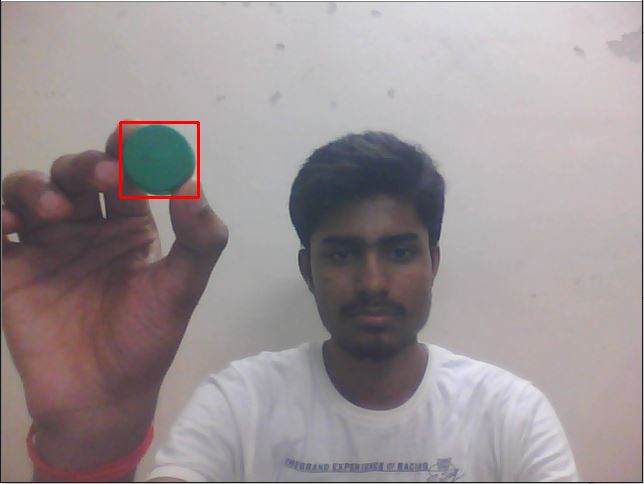
\includegraphics[scale=0.2]{image1.jpg}
			\end{center}
			\begin{center}
				Figure: Colored object tracking using HSV.
			\end{center}
		\end{figure}
	\end{itemize}
\end{frame}
\begin{frame}{Tasks Accomplised}
	\begin{itemize}		
		\item \textbf{Object tracking (ROI selection) and Tutorial on algorithm used}
		
		\begin{itemize}
			\item[Result:] Camera tracks object  based on ROI selection.
			
			\item[Procedure:]
			\begin{itemize}
				\item Select ROI using Mouse Event.
				\item Calculate 2D Histogram of ROI.
				\item Calculate Back Projection of Histogram of ROI on the frame.
				\item Use CAMShift algorithm to find Object in Next Frame.
			\end{itemize}
			
			\item[Limitation:]Object can not be re-tracked if it goes outside frame and comes back.
		\end{itemize}
	\end{itemize}
\end{frame}
\begin{frame}{Tasks Accomplised}
	\begin{figure}
		\begin{center}
			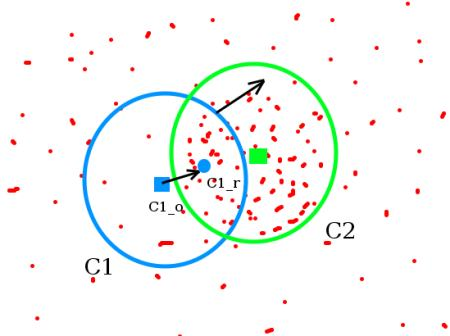
\includegraphics[scale=0.5]{meanshift.jpg}
		\end{center}
		\begin{center}
			Figure: Meansift.
		\end{center}
	\end{figure}
\end{frame}
\begin{frame}{Tasks Accomplised}
	\begin{itemize}		
		\item CAMShift : It applies meanshift first. Once meanshift converges, it updates the size of the window. It also calculates the orientation of best fitting ellipse to it. Again it applies the meanshift with new scaled search window and previous window location. The process is continued until required accuracy is met.
		\begin{figure}
		\begin{center}
			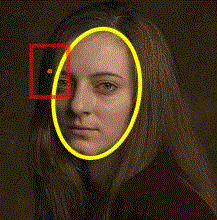
\includegraphics[scale=0.4]{result.png}
		\end{center}
		\begin{center}
			Figure: CAMShift.
		\end{center}
	\end{figure}
	\end{itemize}
\end{frame}
\begin{frame}{Tasks Accomplised}
	\begin{itemize}		
		\item \textbf{Deciding Components of Gimbal and Tutorial on How to make your own Gimbal}
		\begin{itemize}
			\item[Components:]
			\begin{itemize}
				\item Brushless DC Motors.
				\item Brushless Motor Controller.
				\item Damping Shock Absorbing Balls
				\item Shock Absorbing Mounts
				\item Gimbal Motor Frames
				\item Camera Fixing Mount
			\end{itemize}
			\item[Processes:]
			\begin{itemize}
				\item Assembling Gimbal.
				\item Balancing The Gimbal.
			\end{itemize}
		\end{itemize}
	\end{itemize}
\end{frame}
\begin{frame}{Tasks Accomplised}
	\begin{figure}
		\begin{center}
			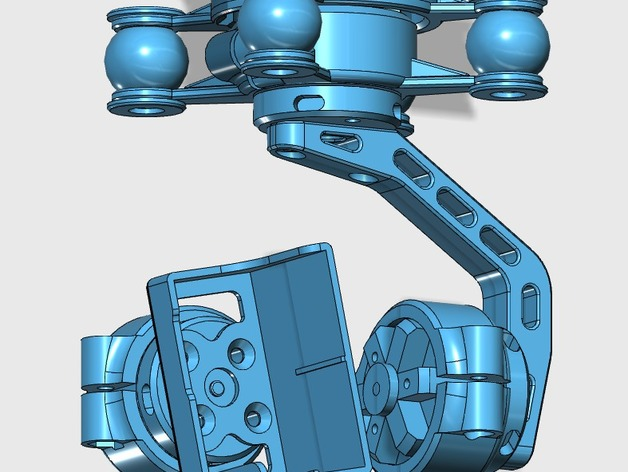
\includegraphics[scale=0.4]{Final_Gimbal.jpg}
		\end{center}
		\begin{center}
			Figure: An assumption of final gimbal.
		\end{center}
	\end{figure}
\end{frame}
\begin{frame}{Tasks Accomplised}
	\begin{itemize}		
		\item \textbf{Setting up the Raspberry Pi}
		\begin{itemize}
			\item Installed Rasbian OS.
			\item Installed OpenCV Library.
			\item Installed other libraries for image processing..
		\end{itemize}
	\end{itemize}
\end{frame}

\section{Challenges Faced}
\begin{frame}{Challenges Faced}
	\begin{itemize}
		\item Making Gimbal with weight constraints and deciding parts.
		\item Selection of a compatible camera.
		\item Tracking of object when the orientation of the object is changed.  
	\end{itemize}
\end{frame}

\section{Future Plans}
\begin{frame}{Future Plans}
	\begin{itemize}
	\item Re-detection of object and Tutorial on algorithms used.
	\item Assembling the camera + gimbal system and interfacing them with the R-Pi.
	\item Keeping the object on the center of the screen by moving the camera.
	\item Object tracking using Pan-tilt camera system.
	\end{itemize}
\end{frame}


\section{Thank You}
\begin{frame}{Thank You}
	\centering THANK YOU !!!
\end{frame}
\end{document}
